\documentclass[12pt]{article}

\usepackage[utf8]{inputenc}
\usepackage[T1]{fontenc}
\usepackage[francais]{babel}
\usepackage{multirow}
\usepackage{array}
\usepackage{color}
\usepackage{stmaryrd}
\usepackage{fancyhdr}
\usepackage{afterpage}
\usepackage{fullpage}
\usepackage{geometry}
\usepackage{setspace}
\usepackage{enumitem}
\usepackage{hyperref}
\usepackage{graphicx}
\usepackage{titling}
\usepackage{float}

% Enlève les contours des liens
\hypersetup{
    linkbordercolor={1 1 1},
    citebordercolor={1 1 1},
    urlbordercolor={1 1 1},
    colorlinks=true,
    linkcolor=black,
    urlcolor=blue
}
\PassOptionsToPackage{hyphens}{url}\usepackage{hyperref}

\pagestyle{fancy}
\setlength{\headheight}{12pt}
\fancyhf{}
\fancyhead[L]{Benoit HOUDAYER, Anthony RUHIER}
\fancyhead[R]{Dawwyd -- Dossier Fonctionnel}
\geometry{headsep=5ex}

\graphicspath{{images/}}


\title{\vspace{-1cm}\textbf{%
    SI75 -- Logiciel de Commande Vocale \vspace{0.5cm}
    \protect\includegraphics[width=4cm]{logo.jpg}\\[0.5em]
    Dossier Fonctionnel}}

\author{Benoit HOUDAYER \\ \href{mailto:benoit.houdayer@utbm.fr}{benoit.houdayer@utbm.fr}
\and Anthony RUHIER \\ \href{mailto:anthony.ruhier@utbm.fr}{anthony.ruhier@utbm.fr}}

\date{23 janvier 2016}
\postauthor{\end{tabular}\vspace{0.6cm} \par Université de Technologie de Belfort-Montbéliard\end{center}}

\begin{document}
    \maketitle
    \thispagestyle{empty}
    \tableofcontents
    \listoffigures

    \section*{Historique des modifications}

    \begin{table}[H]
    \centering

    \begin{tabular}{|l|l|l|l|}
        \hline
        version & date & auteur & modification \\
        \hline
        0.1 & 21 janvier 2016 & BHD & création du document \\
        0.2 & 23 janvier 2016 & ARH & ajout du planing détaillé \\
        \hline
    \end{tabular}
    \end{table}

    \afterpage{\cfoot{\thepage}}
    \newpage

    \section{Fonctionnalités}
    Dawwyd est composé de 3 fonctions principales :
    \begin{description}
        \item[la transcription] est la fonction transformant la voix
            de l'utilisateur en texte, analysable par l'application.
        \item[l'analyse sémantique] est la compréhension du sens de la phrase,
            permettant la prise de décision sur l'action à effectuer.
        \item[l'intégration avec les application de l'utilisateur] réalisée
            grâce à un ensemble de modules, interagissant avec les applications.
            Chaque module implémente une ou plusieurs actions.
    \end{description}

    \subsection{Transcription}
    L'application doit être capable de transcrire
    les paroles de l'utilisateur pour pouvoir interpréter la
    commande
    \begin{itemize}
        \item 60\% de reconnaissance correcte
        \item Possibilité d'effectuer la transcription sur du matériel embarqué
    \end{itemize}

    \subsection{Analyse sémantique}
    Après transcription, une commande doit être interprétée pour déclencher une
    action.
    \begin{itemize}
        \item Choix d'une action en 3 secondes ou moins
    \end{itemize}

    \subsection{Intégration avec les applications de l'utilisateur}
    \paragraph{}
    Les actions à effectuer par Dawwyd auprès des applications de l'utilisateur
    sont matérialisée par des modules. De cette façon, il est possible
    d'intégrer plus facilement de nouvelles fonctionnalités.

    \paragraph{}
    Les modules ne sont pas critiques pour le fonctionnement de l'application
    mais enrichissent simplement l'expérience utilisateur. Pour
    cette raison, la quantité de modules implémentés dépendra de la rapidité
    de l'avancement du projet.

    \paragraph{}
    Au démarrage, Dawwyd devra découvrir les applications installées de façon à
    ne charger que les modules qui seront utilisables par l'utilisateur. Il est
    inutile de charger un module gérant une application absente.

    \subsubsection{Lecteur de musique}
    L'intégration à pour but de couvrir les fonctionnalités pour une utilisation
    basique du lecteur; le but étant de permettre la navigation dans un album
    une fois la lecture lancée manuellement par l'utilisateur.

    \paragraph{}
    Ainsi, les fonctions implémentées seront :
    \begin{itemize}
        \item piste suivante/précédente
        \item lecture/pause
        \item augmenter/diminuer le volume
    \end{itemize}

    \paragraph{}
    Les contraintes associées sont :
    \begin{itemize}
        \item les probabilités de succès de la reconnaissance vocale devront
            tenir les 60\% annoncés plus haut, malgré le bruit ambiant dégagé
            par la musique.
    \end{itemize}

    \subsubsection{Navigateur internet}
    Cette intégration permettra de demander l'ouverture du navigateur sur une
    page précise.

    \begin{itemize}
        \item la page à ouvrir est précisée dans la commande vocale de l'utilisateur
    \end{itemize}

    \paragraph{}
    Ce qui conduit à fixer les contraintes suivantes:
    \begin{itemize}
        \item l'url (l'adresse complète du site à atteindre) ne devra pas être
            dictée entièrement par l'utilisateur, mais fonctionnera par alias.
        \item ouvrir un onglet sur le navigateur par défaut
    \end{itemize}

    \subsubsection{Météo}
    \paragraph{}
    Ce module récupère les informations sur la météo et les énonce à
    l'utilisateur.

    \begin{itemize}
        \item Dawwyd récupère les informations sur la ville de résidence de
            l'utilisateur
        \item les informations sont énoncées de manière concise et
            compréhensible
    \end{itemize}

    \subsubsection{Actualités}
    \paragraph{}
    Dawwyd récupère les titres de l'actualité et les énonce à l'utilisateur.

    \begin{itemize}
        \item les titres sont lus dans l'ordre chronologique à l'utilisateur
            compréhensible
    \end{itemize}


    \section{Enchainement des activités}

    Dawwyd ne possède pas d'interface graphique, ses interactions avec
    l'utilisateur se font uniquement sous forme de réponses sonores
    ou éventuellement de notifications discrètes.

    \begin{figure}
        \centering
        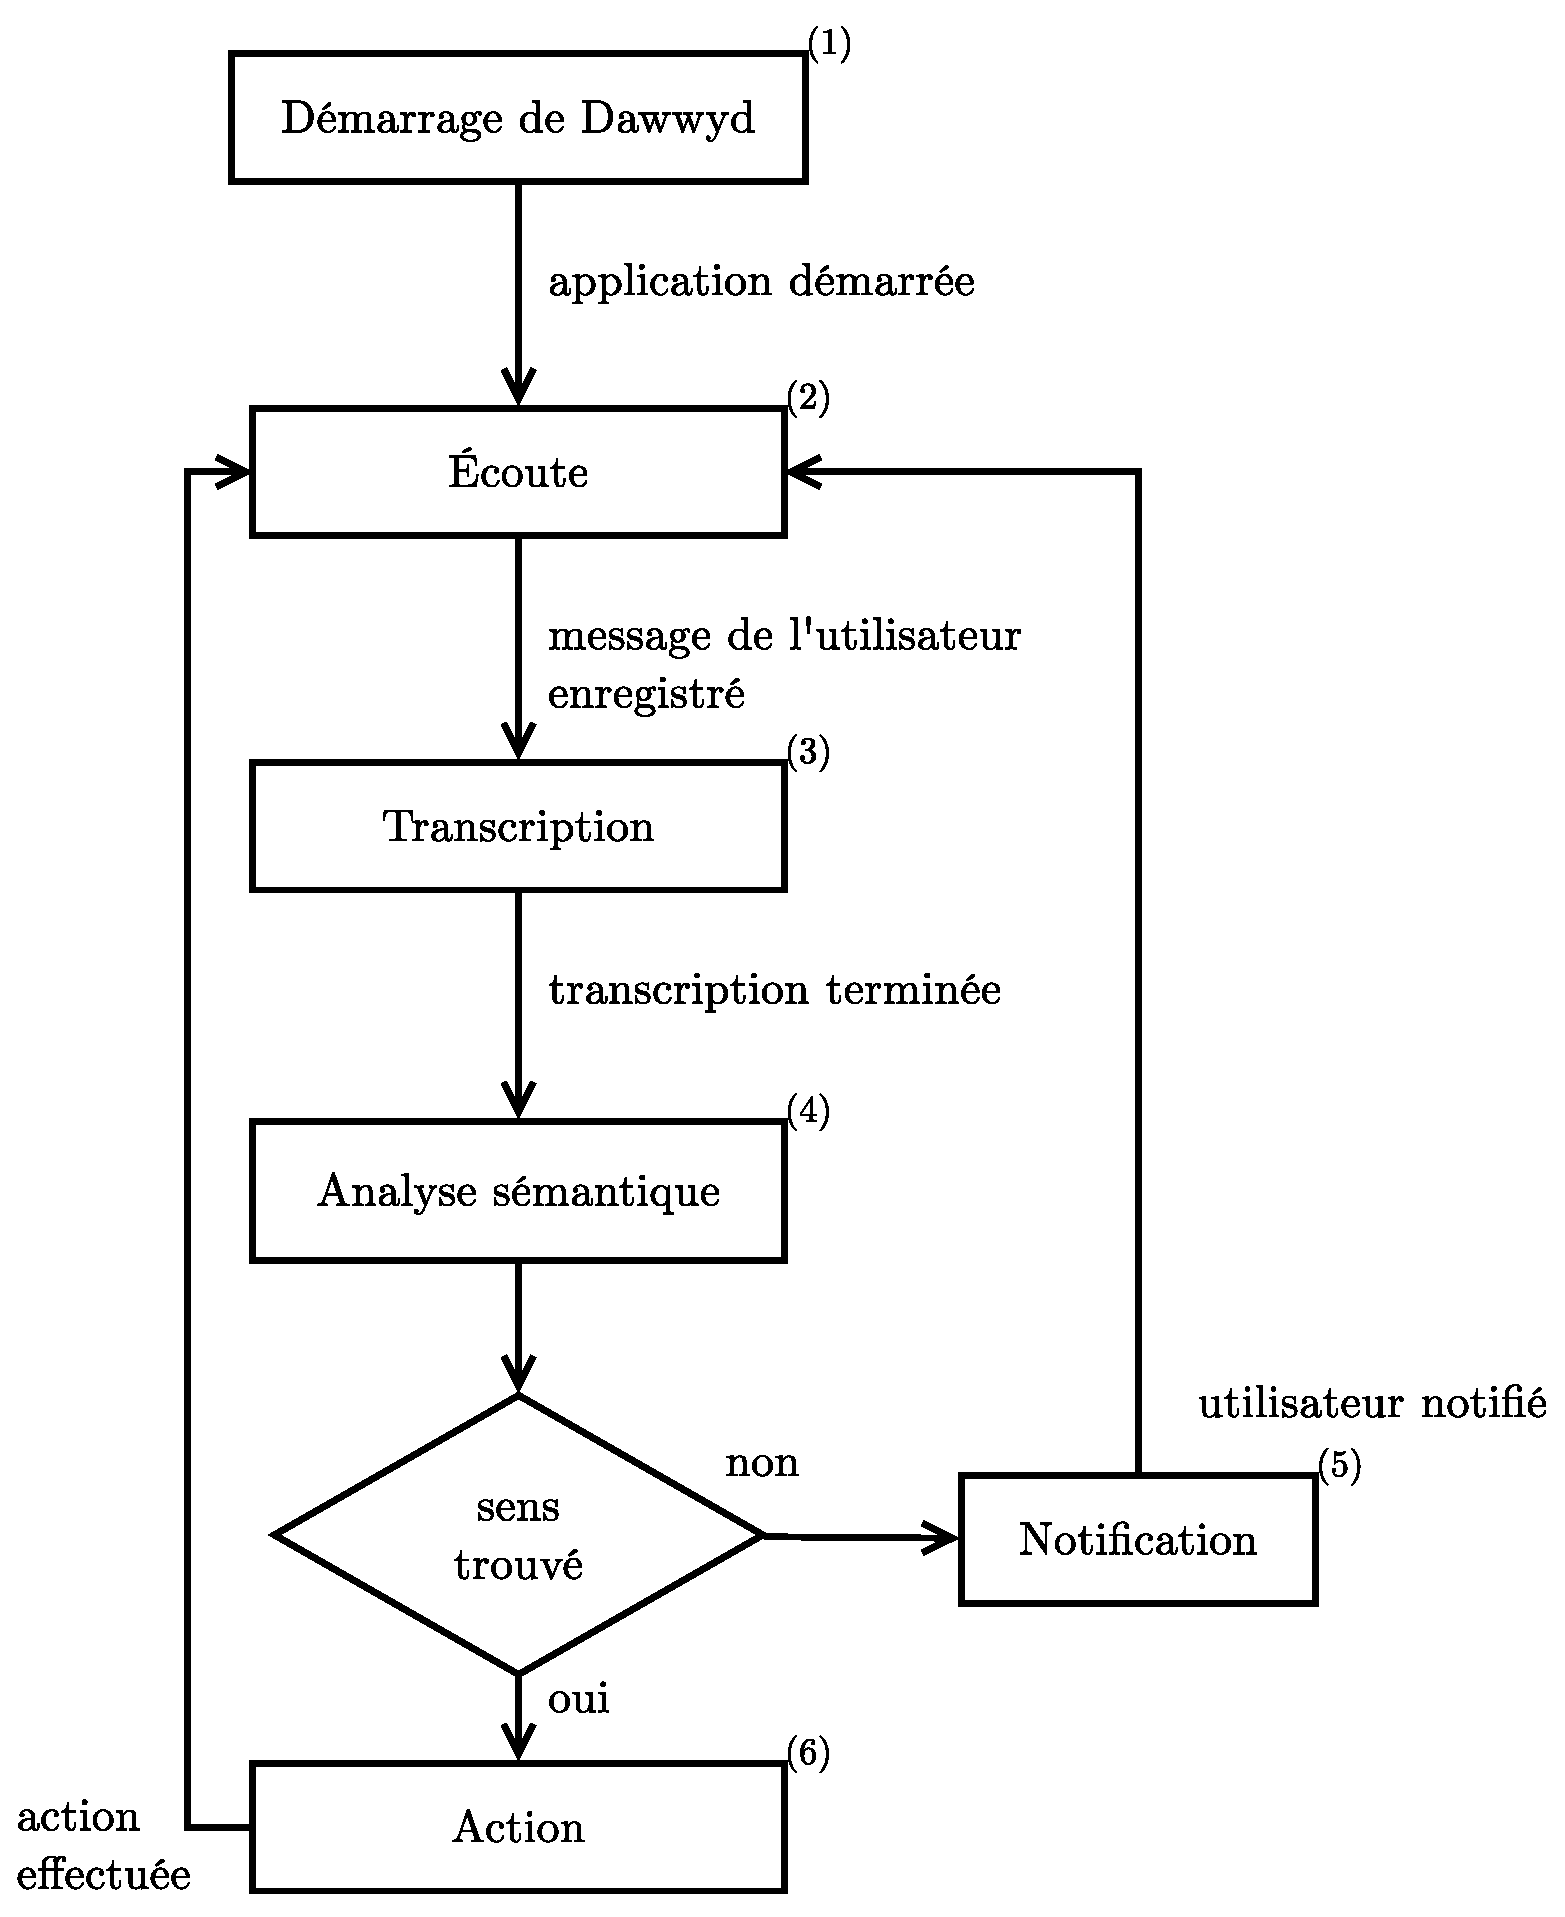
\includegraphics[height=15cm]{diagramme_flux.eps}
        \caption{Flux des activités}
    \end{figure}

    \begin{figure}
        \centering
        \includegraphics[height=1cm]{exemple_notif.png}
        \caption{Exemple de notification}
    \end{figure}

    \paragraph{}
    Description des activités :
    \begin{enumerate}
        \item Dawwyd est démarré par l'utilisateur ou bien automatiquement par
            le système.
        \item Une notification est envoyée à l'utilisateur pour lui signaler
            que l'écoute à démarré. L'enregistrement d'un message provoque
            l'étape suivante.
        \item L'enregistrement de la voix de l'utilisateur est transcrit.
        \item L'analyse sémantique est effectuée et le choix de l'action à effectuer
            est pris dans le temps imparti.
        \item Si aucune action ne correspond à la commande de l'utilisateur,
            Dawwyd signale l'erreur via une notification ou un signal sonore
            puis retourne en phase d'écoute.
        \item Si une action correspond à la commande de l'utilisateur, elle est
            effectuée et Dawwyd retourne immédiatement en phase d'écoute.
    \end{enumerate}



    \section{Planing}

    \begin{figure}[H]
        \centering
        \includegraphics[width=6cm]{gantt.png}
        \caption{Planing détaillé}
    \end{figure}

\end{document}
